\subsection{Emulation Performance Evaluation}

%This chapter presents the evaluation of MCRP. The experiment set ups for Cooja simulation is explained below. In Cooja simulation, interference is introduced. MCRP is evaluated using an end-to-end packet delivery performance metric. The results from the experiments are presented and discussed. 

%///////simulation

%\begin{figure}
%\centering
%\includegraphics[trim=4cm 6cm 2cm 2cm, clip=true, width=0.38\textheight]
%{figures/simulationLayout.pdf}
%\caption{Layout of the simulation nodes}
%\label{fig_simulation}
%\end{figure}

MCRP is evaluated in the Cooja network emulator. 
%Figure \ref{fig_simulation} shows the layout of the network.
The network consists of 31 nodes which are used to run the simulation where one node is used as the border router node, 16 interference nodes, and 14 duty cycled nodes that act as UDP clients to send packets to LPBR spanning over 20-30 metres between each node. RPL border router is used as LPBR in order to move most processing decisions on a PC as it has more RAM and better processing capabilities than a sensor.
The border router also acts as the root of the tree.

In Cooja emulator, an interference model is used to allow full control over the test environment and the experiments are repeatable. Although the interference model does not fully mimic the behaviour of the real world interference, it enables MCRP performance to be tested in various conditions when the channel performance is degraded and to have a better understanding of the performance.

%MCRP is evaluated in the Cooja simulated environment with emulation of TMote sky nodes that feature the CC2420 transceiver, a 802.15.4 radio. The nodes run on IPv6, using UDP with standard RPL and 6LoWPAN protocols. Figure \ref{fig_simulation} shows the layout of the network. The network consists of 31 nodes which are used to run the simulation where one node is used as the border router node, 16 interference nodes, and 14 duty cycled nodes that act as UDP clients to send packets to LPBR spanning over 20-30 metres between each node. RPL border router is used as LPBR in order to move most processing decisions on a PC as it has more RAM and better processing capabilities than a sensor. TelosB sensor has limited RAM and ROM of 10K bytes and 48K bytes of flash memory \cite{telosb-datasheet}. By using a border router, this allows channel changing to be decided in real time without draining the memory and battery on a sensor. The border router also acts as the root of the tree.

%\begin{figure}
%\centering
%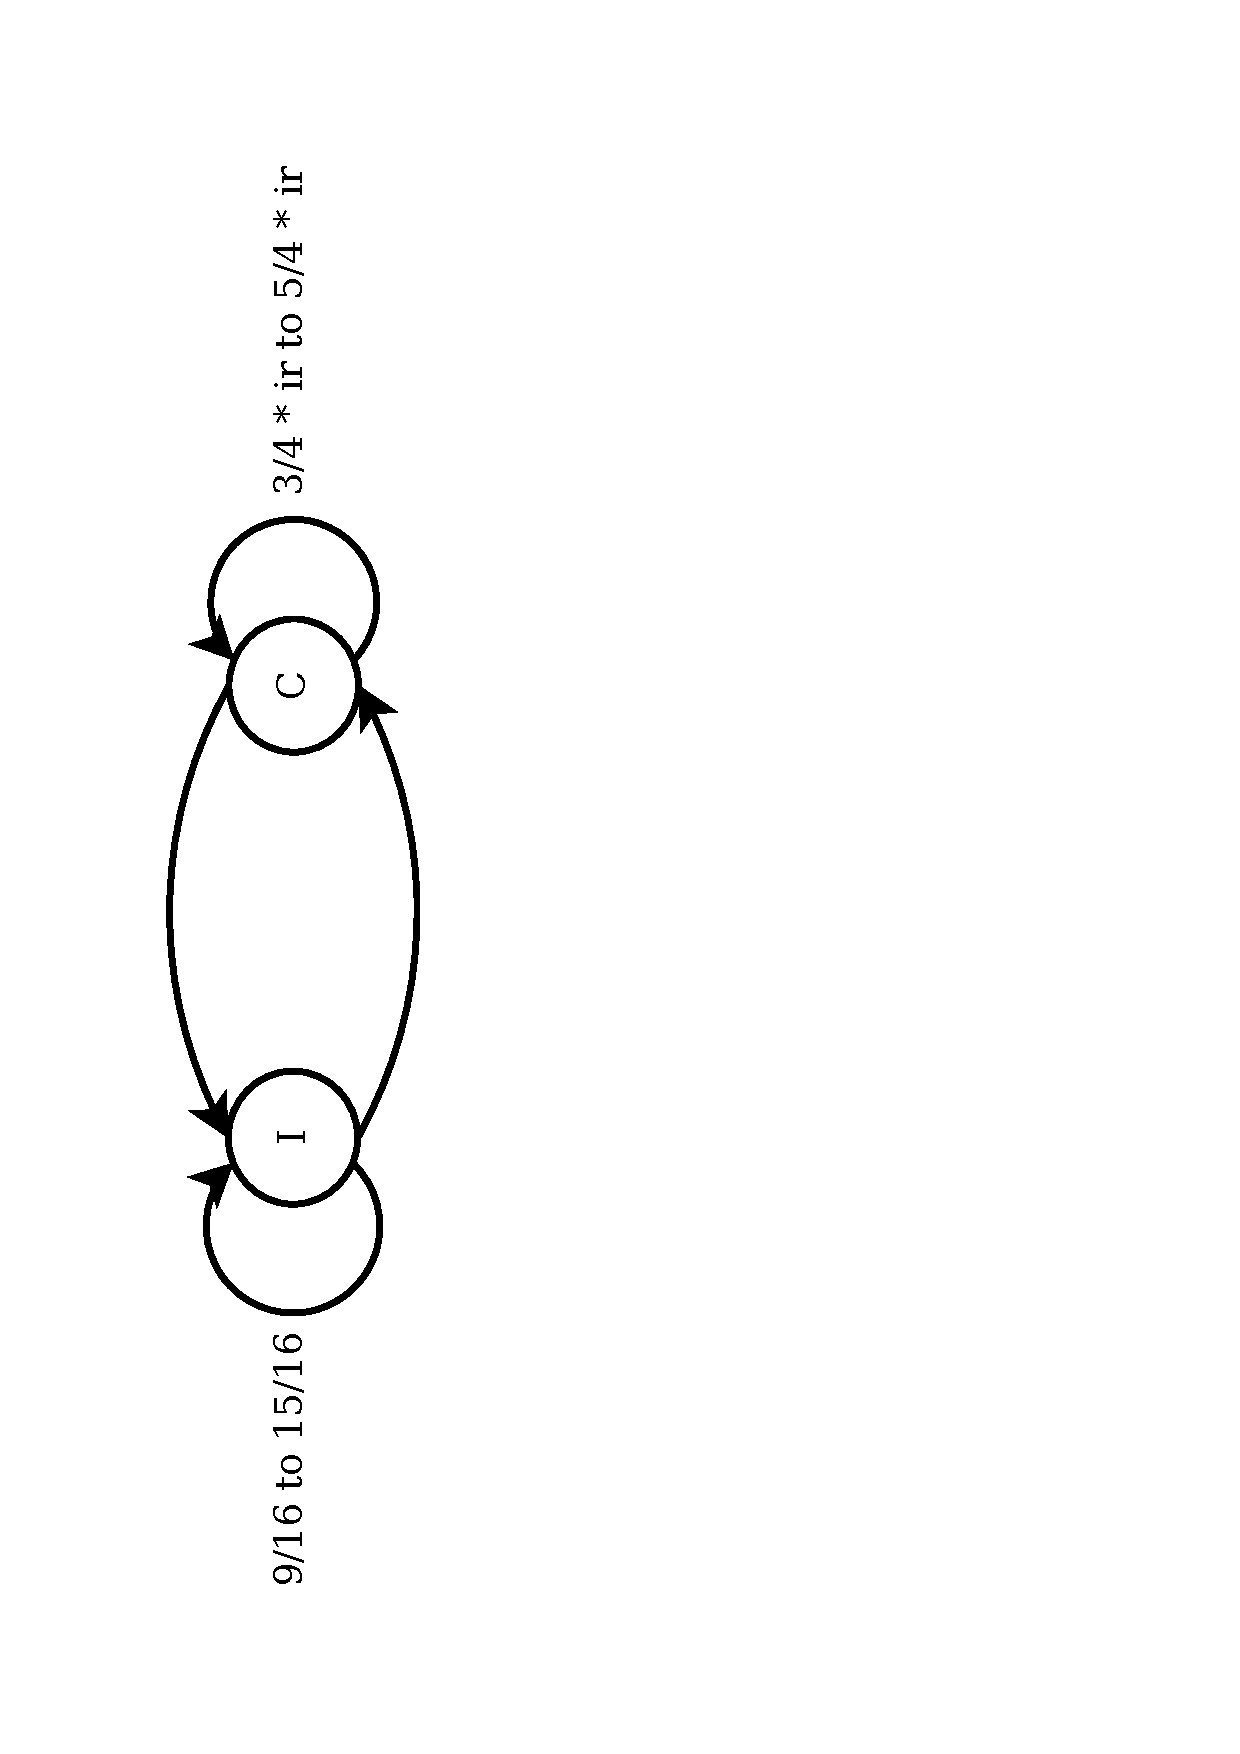
\includegraphics[trim=2cm 2cm 13cm 2cm, clip=true, totalheight=0.36\textheight, angle=270]{figures/interferenceModel2.pdf}
%\caption{Interference model}
%\label{fig_interferenceModel}
%\end{figure}

The controlled interference node generates semi-periodic bursty interference is simulated to resemble a simplified Wi-Fi or Bluetooth transmitter on several channels at random. The interference model proposed in \cite{interferenceModel} is used in the simulation to generate similar packet loss rate to the theoretical and real nodes values given in \cite{radio2009}. The interference has two states, a clear state (C) and an interference state (I). 
In the interference state, the interference node generates packets for a time that is uniformly distributed between $9/16$ seconds and $15/16$ seconds. In the clear state the interferer produces no packets and stays in this state for between $3/4 * \emph{clear\textunderscore time}$ and $5/4 * \emph{clear\textunderscore time}$ where \emph{clear\textunderscore time} refers to the rate of interference (ir). 
%The model is illustrated in Figure \ref{fig_interferenceModel}.
Multiple channels interference is used in the simulation to show the hypothesis that MCRP can help avoid interference. The scenario that is considered is where ContikiMAC with RPL system is subject to interference on its channel after set up has successfully completed so the RPL set up is allowed to complete before interference begins.

The protocol performance in loss over time in the presence of interference is observed. The level of interference used in term of the \textit{clear\_time} is 100\% for no interference, 75\% for mild, 50\% for moderate and 25\% for extreme interference. The percentage represents the ratio of the time the channel is clear for transmission.
%Two multiple channels interference scenarios are considered; (i) extreme and no interference rate on 8 channels each and (ii) extreme, moderate, mild and no interference rate on 4 channels each.
The interference channels are randomly chosen from the available 16 channels.
% and the same interference channels and rates are used throughout the experiments. 
However, channel 26 is kept clear from interference in order to ensure RPL set up is unaffected. 
%In scenario 1, the interference rates are fixed to extreme and no interference to observe the effect it has on the channel changing decisions. In scenario 2, the interference rates are vary to observe how MCRP copes in deciding a channel when there is more interference than scenario 1 but with less interference intensity. 
The emulation runs for a duration of 45-60 minutes to send 210-560 packets. When the nodes are switched on for the first time, all nodes are initialised to channel 26, the default channel for Contiki MAC layer. RPL is allowed five minutes to set up (which is ample time). RPL topology is formed in a minute. The simulation waits for another five minutes to allow trickle timer to double the interval length so that RPL control messages are not being sent frequently. The multichannel protocol is then runs for 25 minutes. In the 15 nodes simulation, the protocol takes 20-25 minutes to run the channel change set up. Another 5 minutes wait time is allowed if retransmissions happen. 
%In a single channel simulation, all the nodes are changed to channel 22 after 5 minutes of RPL set up time. This allows RPL to have enough time to discover all nodes to form an optimised topology. The topology formation does not form completely if the interference node interferes from the beginning. 

The interference node starts sending packets to interfere after 3 minutes the system is switched on so that the interference channel is involve in the channel changes decision. It is proven that the protocol tries to avoid changing to the interference channel through time out and probing failures. After 30 minutes, the client nodes will send a normal packet periodically every 30-60 seconds to LPBR. This is done in order to avoid collision of the nodes sending at the same time. 

%\subsection{Simulation Results}
The performance of MCRP is compared against the standard ContikiMAC with RPL and Orchestra to demonstrates MCRP abilities in dealing with external and intra interferences. Orchestra does not support RPL downwards routing due to limited memory in TelosB. It however, support the upwards traffic which is require in the experiments as all traffics are directed upwards towards the LPBR.
MCRP is analysed using an end-to-end packet delivery performance metric, setup overhead, channel switching and reconnection delay in MCRP. The transmission success rate is calculated from the sender to the receiver over multiple hops. 
The simulations are repeated ten times. In all plots, the mean value of the ten simulations is plotted with error bars corresponding to one standard deviation in either deviation to give a measure of repeatability. The plots are of the proportion of received packets (from 0\% to 100\%) against time where the loss is measured over the previous time period.  The x-value is shifted slightly left and right to prevent error bars overlapping.


%%This chapter demonstrates MCRP abilities in dealing with external and internal interferences. MCRP is tested in the simulated environment to study the effect of multichannel to the performance in a controlled environment. MCRP results are compared to the standard single channel ContikiMAC and multichannel Orchestra that implemented TSCH in term of the end-to-end packet delivery. The setup overhead, channel switching and reconnection delay in MCRP are discussed to prove that these values are negligible in the context of WSNs that could run in years while maintaining high throughput.

\subsubsection{Packet Loss Rates}
%%repeatition of what already explained
%The performance obtained in ContikiMAC with RPL (single channel) is compared with MCRP in terms of packet loss rate.
%As described previously, levels of interference used (referred to as \emph{clear\textunderscore time} in \cite{interferenceModel}) vary among 100\% (no interference), 75\% (mild), 50\% (moderate) and 25\% (extreme) where the percentage is the ratio of the time the channel is clear for transmission. All of the tests have a common format: the RPL procedure is allowed to set up without interference in order not to bias subsequent tests.
%Then the interferers begin to operate with a constant level (none, mild, moderate or extreme).

\begin{figure}
\centering
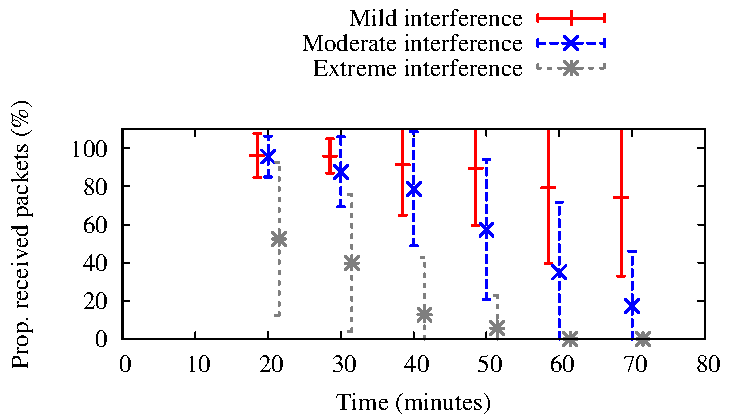
\includegraphics[width=0.45\textwidth]{figures/single_channel.pdf}
\caption{Emulations: Level of packet loss for mild, moderate and extreme interference levels using single channel}
\label{fig:interference}
\end{figure}

Figure \ref{fig:interference} shows the results in emulation for ContikiMAC with RPL protocol. It can be seen that the level of packet loss varies considerably between experiments (the error bars are always large). It can also be seen that even for mild interference there is considerable loss and this gets worse as time proceeds. In the extreme interference case the loss always goes up until no packets are received. For mild interference the system evolves until it is losing around 20\% of packets but this can increase.

In the single channel, the node does not have enough time to recover from the interference to retransmit and drops all packets. In the extreme interference case, it shows that there are more packets drop over time and it stops receiving packets as it doesn't have enough buffer to store the incoming packet and the channel becomes congested. However, as the interference rate increases (less interference), the single channel performance improves as it has more time to recover.

\begin{figure}
\centering
\subfigure[Fixed layout]
{\label{fig:randomInterference}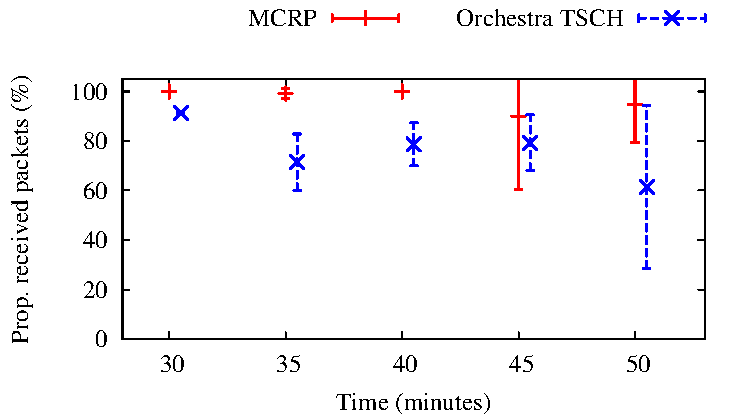
\includegraphics[width=0.45\textwidth]{figures/ri.pdf}}
\subfigure[Random layout]
{\label{fig:randomAll}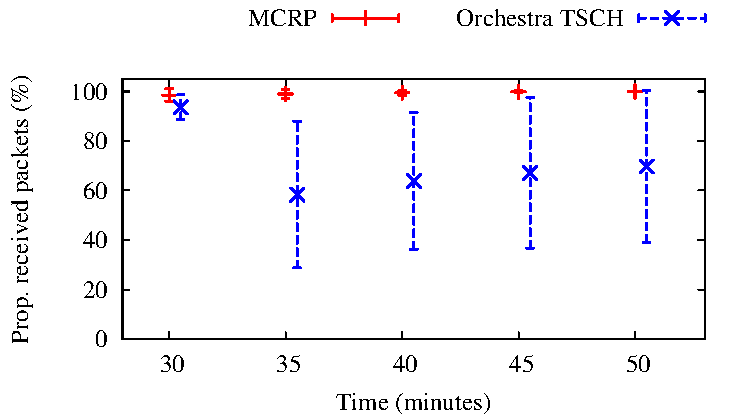
\includegraphics[width=0.45\textwidth]{figures/ra.pdf}}
\caption{Emulations: Level of packet loss for MCRP and Orchestra}
\label{fig:layouts}
\end{figure}


To evaluate MCRP capabilities to cope with interference from many sources, thus channels, and to compare to an existing multichannel protocol Orchestra, the emulations were run where (i) the layout is fixed while the interference channels are chosen by random and (ii) all the nodes including the interference nodes are placed randomly. 
In the experiments, Orchestra uses channel hopping on all 16 channels.  

Figure \ref{fig:layouts} show MCRP and Orchestra results for the fixed and random nodes layouts.
MCRP performs extremely well in both scenarios as the average packet reception rates are between 90\%-100\% and the protocol successfully detects the channels with interference.
Orchestra has higher packet loss compared to MCRP, showing a maximum of 40\% packet loss on average as the channels with interference are being used for transmission periodically.
%around 90-100\% received packet as it hops on all channels which includes the channels that have higher interference. 
In comparison, MCRP selects certain channels to change into after checking the channels condition which gives MCRP a smaller number of packet loss.
MCRP avoids the interference channel while Orchestra hops to the next channel in the next iteration for transmission.

%single channel, two interference scenarios are considered.
%In scenario 1 half the channels (including the original channel) have no interference at all and half the channels have extreme interference.
%In scenario 2, four channels (including the original channel) have no interference, four have mild, four moderate and four extreme interference. Figure \ref{fig:multi_interference} shows multichannel results for these two scenarios. In scenario 1 the protocol performs extremely well, the packet loss is near zero and the protocol successfully detects channels with interference.
%Scenario 2 has similar results as in scenario 1. The protocol does well at reducing the effects of interference and could detect moderate and mild interference.
%MCRP avoids the interference channel which resulted in less loss than in Orchestra. 

%Orchestra shows good result as it hops to another channel in the next iteration which allows it to move from the interference channel faster to be able to keep the loss rate to a minimum. While Orchestra has high proportion of received packets, MCRP shows near 100\% packet reception. 
%Orchestra shows no deviation as the channel values are fixed for each iteration thus giving the same results each time unlike MCRP where the channels are selected at random before it is used.

%In scenario 2 where there are mild interference channels, most of the probing messages on those channels are received. This means that the channels can be used for transmission. This is also the case with a single channel. The interference does not affect the transmissions as the interference is not frequent enough. The node has enough time to recover from the interference through retransmissions. However, the interference would slightly effect the packet transmission over time. 

%\begin{figure}
%\centering
%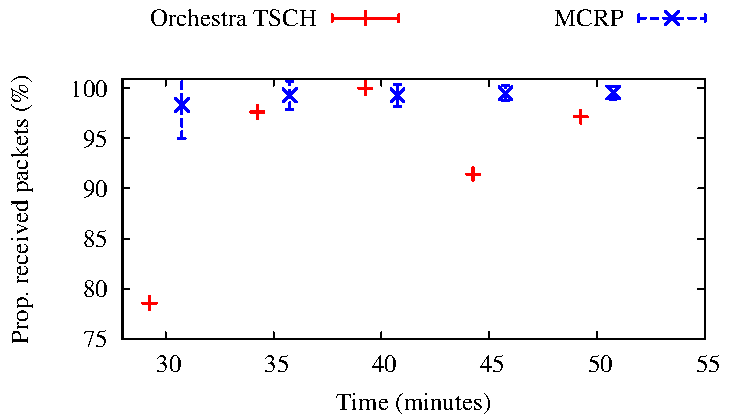
\includegraphics[width=0.45\textwidth]{figures/tsch1.pdf}
%\caption{Level of packet loss on testbed for MCRP and Orchestra}
%\label{fig:orchestra_sim}
%\end{figure}

%To prove that MCRP also performs better than not only single channel protocol, MCRP is compared against Orchestra. In the experiment, Orchesta uses channel hopping on all 16 channels. Figure \ref{fig:orchestra_sim} shows the result from scenario 2 on both MCRP and Orchestra. Orchestra has a low packet loss showing around 90-100\% received packet as it hops on all channels which includes the channels that have higher interference. In comparison, MCRP selects certain channels to change into after checking the channels condition which gives MCRP nearly zero packet loss. Orchestra shows good result as it hops to another channel in the next iteration which allows it to move from the interference channel faster to be able to keep the loss rate to a minimum. While Orchestra has high proportion of received packets, MCRP shows near 100\% packet reception. Orchestra shows no deviation as the channel values are fixed for each iteration thus giving the same results each time unlike MCRP where the channels are selected at random before it is used.


\subsubsection{Setup Overhead}
Obviously the system of changing channels and probing to see if a channel is free of interference introduces a certain amount of overhead into
the protocol. This takes the form of (a) extra messages passed and (b) extra time taken to set up. Default RPL on ContikiMAC for the topology considered in these experiments completed its set up using 276 packets. MCRP, the multi-channel protocol completed its set up in 716 packets, that is an overhead of 440 packets on top of RPL. 
This overhead comes from the channel changing messages to nodes and neighbours, probing messages, channel confirmation messages and acknowledgement packets which are required to ensure a thorough channel change decision.
However, it is worth mentioning that this is a one-off cost. This represents (in this experimental set up) approximately one hour of extra packets in the situation of a deployment that is meant to work for weeks or months.  In terms of set up time, the protocol begins to change channels only when the RPL set up process is complete (or at least stabilises). The set up time is 1154 seconds beyond the RPL set up time of 286 seconds. However, it should be noted that, in fact, the system remains fully functional and capable of sending packets during the set up so this set up overhead does not matter to data transmission.
Therefore it can be concluded that data sending costs (extra packets) of set up are negligible in the context of a deployment that will last more than a day. The extra set up time is also negligible within this context and furthermore does not degrade performance of the network during this set up phase.

\subsubsection{Channel Switching Delay}
Each node has different listening and transmitting channels. When the node is awake, it waits for incoming packets on its listening channel. If the node has a packet to send, it will switch to the next hop listening channel based on the channel information from the neighbour table. The channel switching takes at most 100$\mu$ to switch to the transmission channel. This delay is negligible in the low packet rate WSN. MCRP ContikiMAC uses a transmission phase-lock where the transmission node knows the receiver wake up phase. The node starts transmitting just before the receiver is expected to be awake. The channel switching happens shortly before the receiver is ready to receive the packets, thus the time taken in channel switching does not affect the packet reception.
The node goes back to sleep once the transmission has succeeded or reached the maximum number of retransmissions (packet loss). In the next iteration, the node is reset and wakes up on its listening channel. 

The channel reset is done in these cases: (i) the queue buffer is empty, (ii) before sending the next packet from the queue buffer, and (iii) the last packet in the queue buffer has been sent. This reset is done to avoid any delay in packet reception that could happen when the node is awake.

\subsubsection{MCRP Reconnection}

\begin{figure}
\centering
\subfigure[Initial tree]{\label{fig:r1}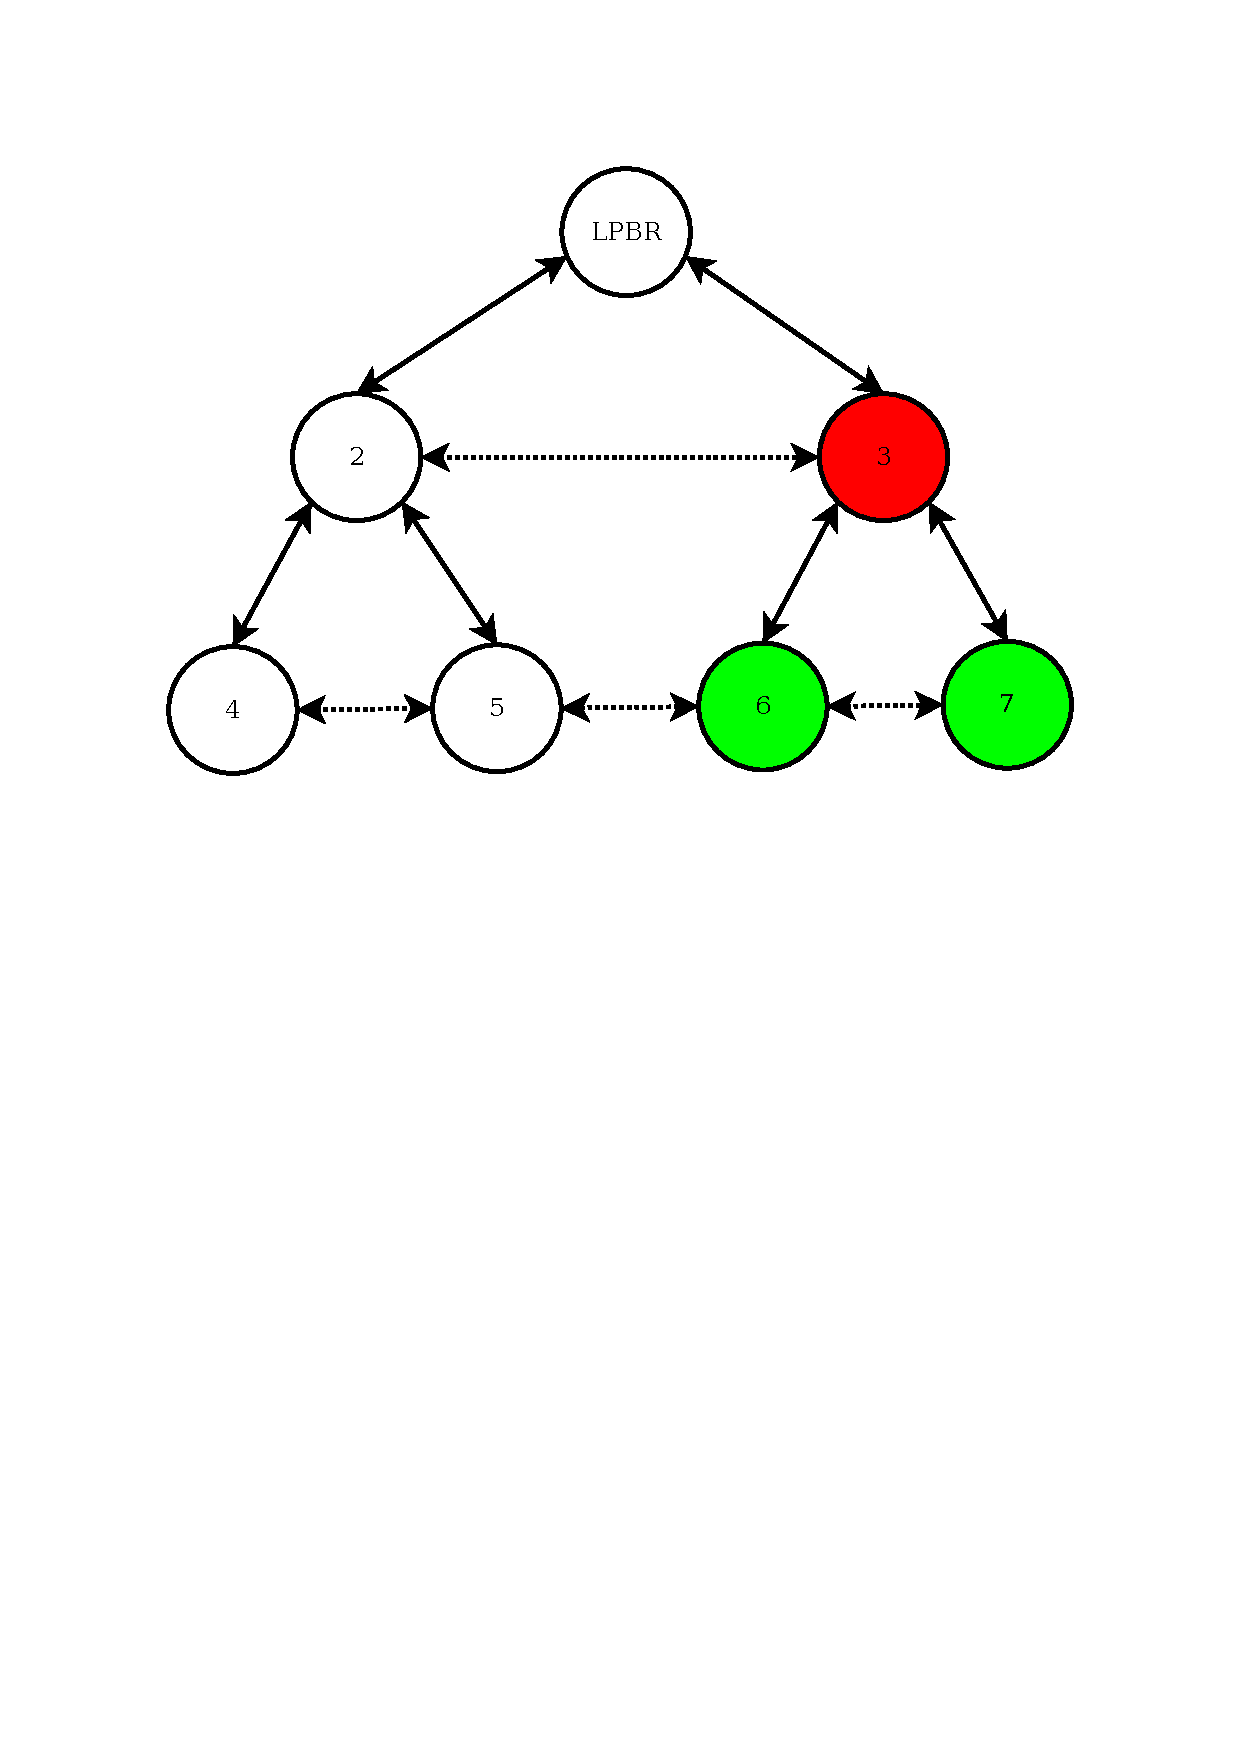
\includegraphics[trim=2cm 16cm 2cm 2cm, clip=true, totalheight=0.12\textheight]
{figures/reconnection1.pdf}}        
\hfill        
\subfigure[Reconstructed tree when node 3 is undetected]{\label{fig:r2}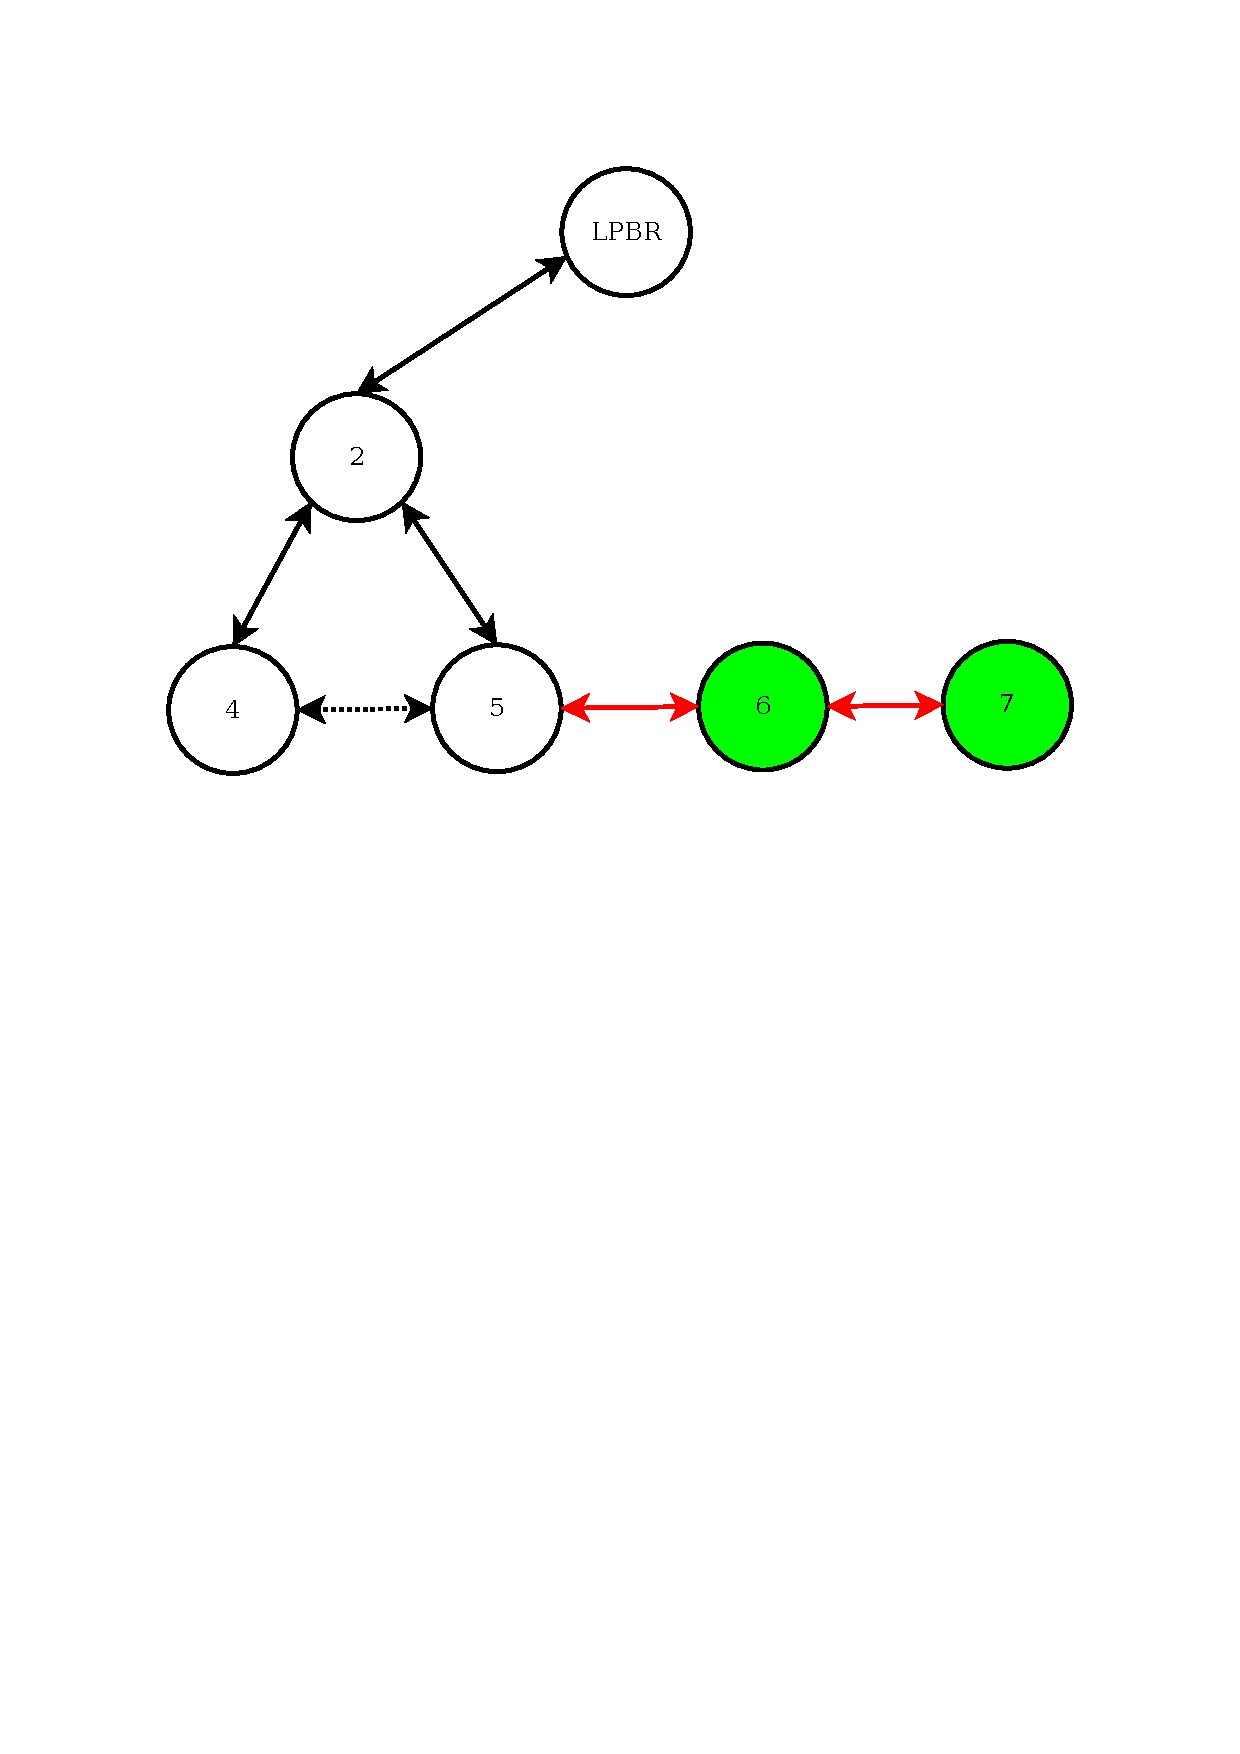
\includegraphics[trim=2cm 16cm 2cm 2cm, clip=true, totalheight=0.12\textheight]
{figures/reconnection2.pdf}}
\caption{A simple tree to emulate the tree reconnection}
\label{fig:reconnectionLayout}
\end{figure}

\begin{figure}
\centering
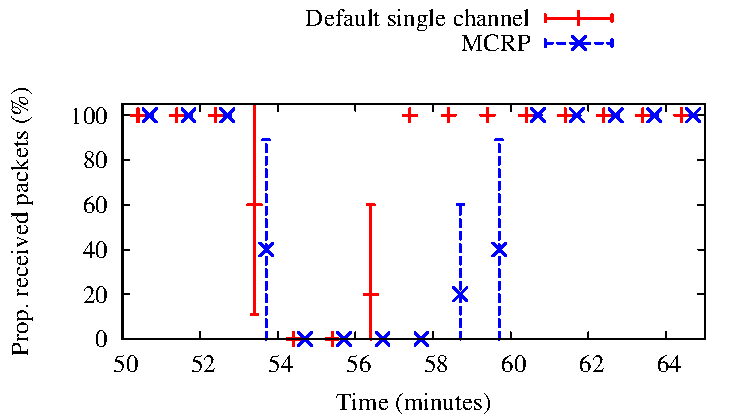
\includegraphics[width=0.45\textwidth]{figures/reconnect.pdf}
\caption{Emulations: Reconnection time taken for MCRP and single channel}
\label{fig:reconnection}
\end{figure}

%In this thesis, the nodes are assumed to be static. The location and the number of nodes are constant. However, for future improvement, MCRP needs to be able to adapt to mobile network and additional nodes after the initial run time. MCRP results in detecting and adjusting the routes are compared with a single case scenario. 

Figure \ref{fig:reconnectionLayout} shows the experimental setup to test MCRP reconnection in term of the time taken to detect and adjust the routes when a node fails (run out of battery or cannot be detected). There is no external interference introduced to ensure an accurate convergence time of the topology. The dotted lines represent potential paths and the solid lines are the selected paths. The result from MCRP is compared to a single case scenario with the same setup.
%Each node sends 25 packets before a node becomes dysfunctional.
In the figure, node 3 is disabled after 53-54 minutes (25 packets are sent and received). Node 6 and 7 route through node 3 to the LPBR. When node 3 is dropped, node 6 and 7 have to find another route which is through node 5 and 2 to get to the LPBR. The time taken for the nodes to reconfigure the routes and the number of packet loss are showed in Figure \ref{fig:reconnection}. 

In MCRP, it took between 5-7 minutes before node 6 and 7 discover and reconnect with the tree to proceed with the transmission. Single channel however, was slightly quicker, taken 3-5 minutes. The reason for this is MCRP control packets are sent on several channels, thus it would take slightly longer to be able to reach all nearby nodes that might be on different listening channels. A single channel on the other hand, could send a broadcast to the nodes which help to reduce the time taken during the topology reconnection.
The reconnection time in MCRP is acceptable as MCRP shows high packet reception once the route is discovered in interference cases.

Comparing to Orchestra, Orchestra is a synchronous protocol. It has a dedicated slot and periodic schedule for RPL signalling which means it detects the failed node quicker unlike in MCRP and default single channel asynchronous protocols. The results from the Orchestra simulation shows that as Orchestra has a slot checking the nodes every minute, it is able to reconnect the nodes without having any packet loss. The disadvantages of Orchestra are, the nodes are listening on the same channel during the broadcast which the known channel is prone to attack. Also, even though Orchestra introduces priority to the traffic, RPL traffic is sent frequently at every period if there is no other higher priority traffic. Trickle timer that is used by the default RPL has the advantage of reducing the number of redundant control packets by doubling the waiting time for the control packets. Orchestra detects failed node quicker at the cost of frequent control packets that are redundant in a stable topology which increases the use of bandwidth and nodes energy consumption.

%/////

%This chapter demonstrates MCRP abilities in dealing with external and internal interferences. MCRP is tested in the simulated environment to study the effect of multichannel to the performance in a controlled environment. MCRP results are compared to the standard single channel ContikiMAC and multichannel Orchestra that implemented TSCH in term of the end-to-end packet delivery. The setup overhead, channel switching and reconnection delay in MCRP are discussed to prove that these values are negligible in the context of WSNs that could run in years while maintaining high throughput.